\documentclass{standalone}
\usepackage{tikz}
\usetikzlibrary{trees,positioning}
\definecolor{breastpink}{RGB}{234,128,176}
\usepackage{libertine-otf}
\begin{document}
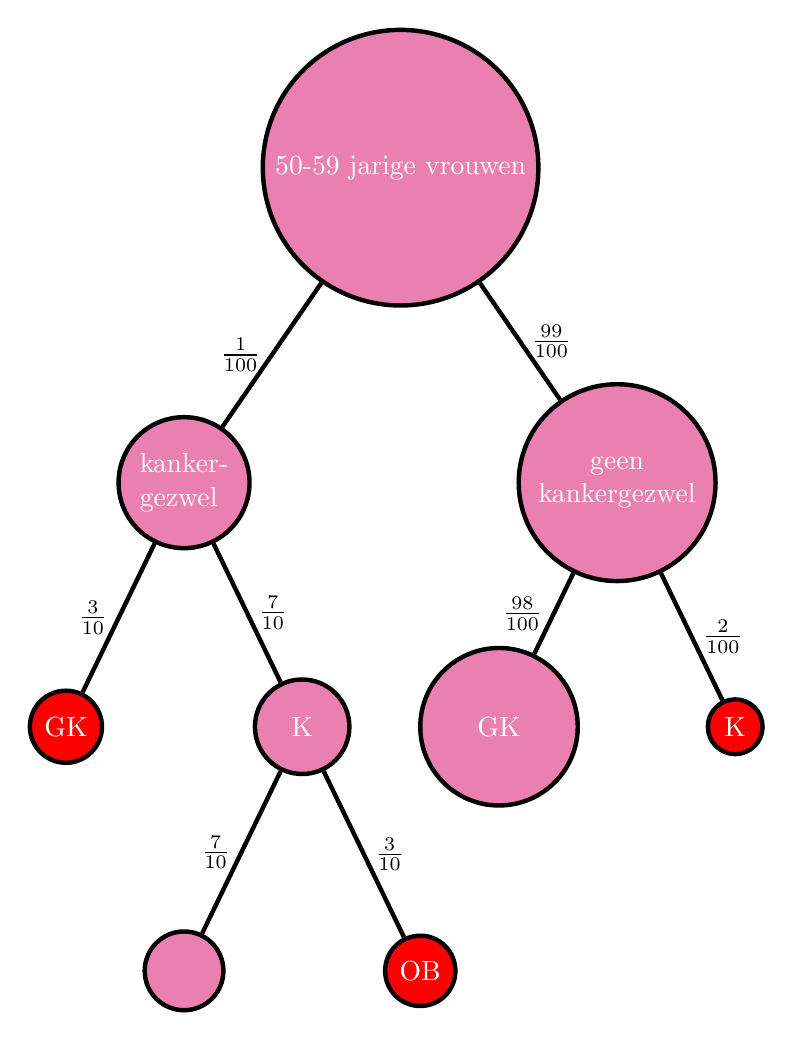
\begin{tikzpicture}[bal/.style={circle,fill=breastpink,minimum size=1.0cm, text=white,draw, ultra thick},level 1/.style={level distance=4cm, sibling distance=5.5cm},
	level 2/.style={sibling distance=3cm,level distance=3.1cm},
	edge from parent/.style={draw,ultra thick}
]
	\node[bal,minimum size=3.5cm] {50-59 jarige vrouwen}
		child {node[bal,minimum size=1.3cm,align=left] {kanker-\\gezwel} 
			child {node[bal,minimum size=0cm,fill=red] {GK}
			edge from parent node[left] {$\frac{3}{10}$}
			}
			child {node[bal,minimum size=1.2cm] {K}
				child {node[bal] {}
			edge from parent node[left] {$\frac{7}{10}$}
				}
				child {node[bal,fill=red,minimum size=0cm] {OB}
			edge from parent node[right] {$\frac{3}{10}$}
				}
			edge from parent node[right] {$\frac{7}{10}$}
			}
			edge from parent node[left] {$\frac{1}{100}$}
		}
		child {node[bal,minimum size=2.5cm,align=center] {geen\\ kankergezwel}
			child {node[bal,minimum size=2.0cm] {GK}
			edge from parent node[left] {$\frac{98}{100}$}
		}
			child {node[bal,minimum size=0cm,fill=red] {K}
			edge from parent node[right] {$\frac{2}{100}$}
			}
			edge from parent node[right] {$\frac{99}{100}$}
		};
\end{tikzpicture}
\end{document}
